\documentclass[12pt]{article}
%	options include 12pt or 11pt or 10pt
%	classes include article, report, book, letter, thesis
\usepackage{amsmath,amsfonts,amssymb}
\usepackage{graphicx}
\usepackage{lipsum}
\usepackage{mwe}
\usepackage{float}
\newcommand\tab[1][1cm]{\hspace*{#1}}
\graphicspath{ {images/} }
\usepackage{hyperref}
\hypersetup{
    colorlinks=true,
    linkcolor=blue,
    filecolor=magenta,      
    urlcolor=cyan,
}
\urlstyle{same}
\begin{document}

\begin{titlepage}
\title{Mining Uber Dataset}
\author{Abhilash Mysore Somashekar \\Raviraj Prakash Wani \\Sanil Jain \\ Satya Akhil Chowdary Kuchipudi }
\date{1 April 2017}
\maketitle
\end{titlepage}


\textbf{Introduction} \\

Uber is a smartphone-app which provides on demand ride service connecting users who need to get somewhere with drivers willing to give them a ride. The service has been hugely controversial, due to regular taxi drivers claiming that it is destroying their livelihoods, and concerns over the lack of regulation of the company?s drivers, surge pricing etc. \\

The business is rooted firmly in Big Data and leveraging this data in a more effective way than traditional taxi firms have managed has played a huge part in its success. Uber?s entire business model is based on the very Big Data principle of crowd sourcing. Anyone with a car who is willing to help someone get to where they want to go can offer to help get them there. \\

FiveThirtyEight obtained the data from the�NYC Limo and Taxi commission by submitting a Freedom of Information Law request on July 20, 2015. The dataset is contains on over 4.5 million Uber pickups in New York City from April to September 2014. This data was used for four FiveThirtyEight stories: Uber Is Serving New York?s Outer Boroughs More Than Taxis Are, Public Transit Should Be Uber?s New Best Friend, Uber Is Taking Millions Of Manhattan Rides Away From Taxis, and Is Uber Making NYC Rush-Hour Traffic Worse? \\

We are extending current analysis using best practices in Data Mining to answer questions like how many pick-ups can we expect on a day, given time and at a location in NYC. We also would analyze ?Hot-Spots?, those are best places for drives to be to get the most pickups during a day. We would be performing Density Estimation, Gaussian Process Regression and also predict ride patterns for weekdays. Extending to this, we may also mine for patterns if weather changes with pickups

\break

\textbf{Exploratory Analysis Goals} \\

\begin{itemize}
	\item Preprocessing of data (rounding of the Latitude and Longitudes)
	\item To find out whether 4.5 million data points over 6 months are continuous or not
	\item To plot counts in histograms as well as plot Uber pickups on actual map and look at the coverage of NYC
	\item Analyze Uber pickup data over various months
	\item Finding the hotspot locations in the data. These are the locations where there are pickups more than a specified threshold
\end{itemize}

\textbf{Graphical Analysis:} \\

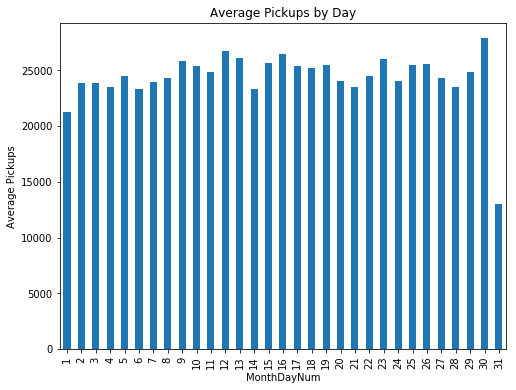
\includegraphics[width=8cm, height=8cm]{ByDay.png}
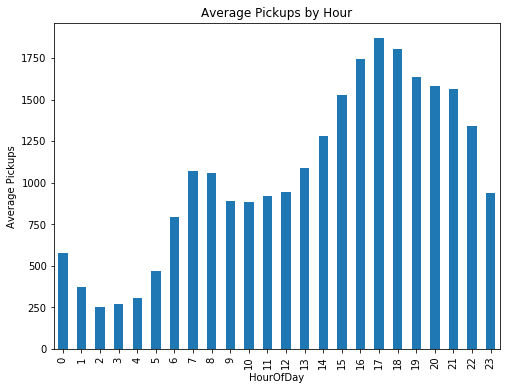
\includegraphics[width=8cm, height=8cm]{ByHour.png}	
\begin{center}
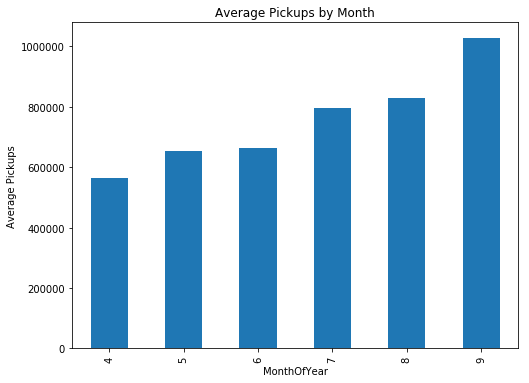
\includegraphics[width=8cm, height=8cm]{ByMonth.png}
\end{center}
\textbf{Geographical Plot (Density Plot):}  \\

The complete density plot carves out the map of New York City on a black canvas by geography. This further strengthens the range of geographical data in dataset.
\begin{center}
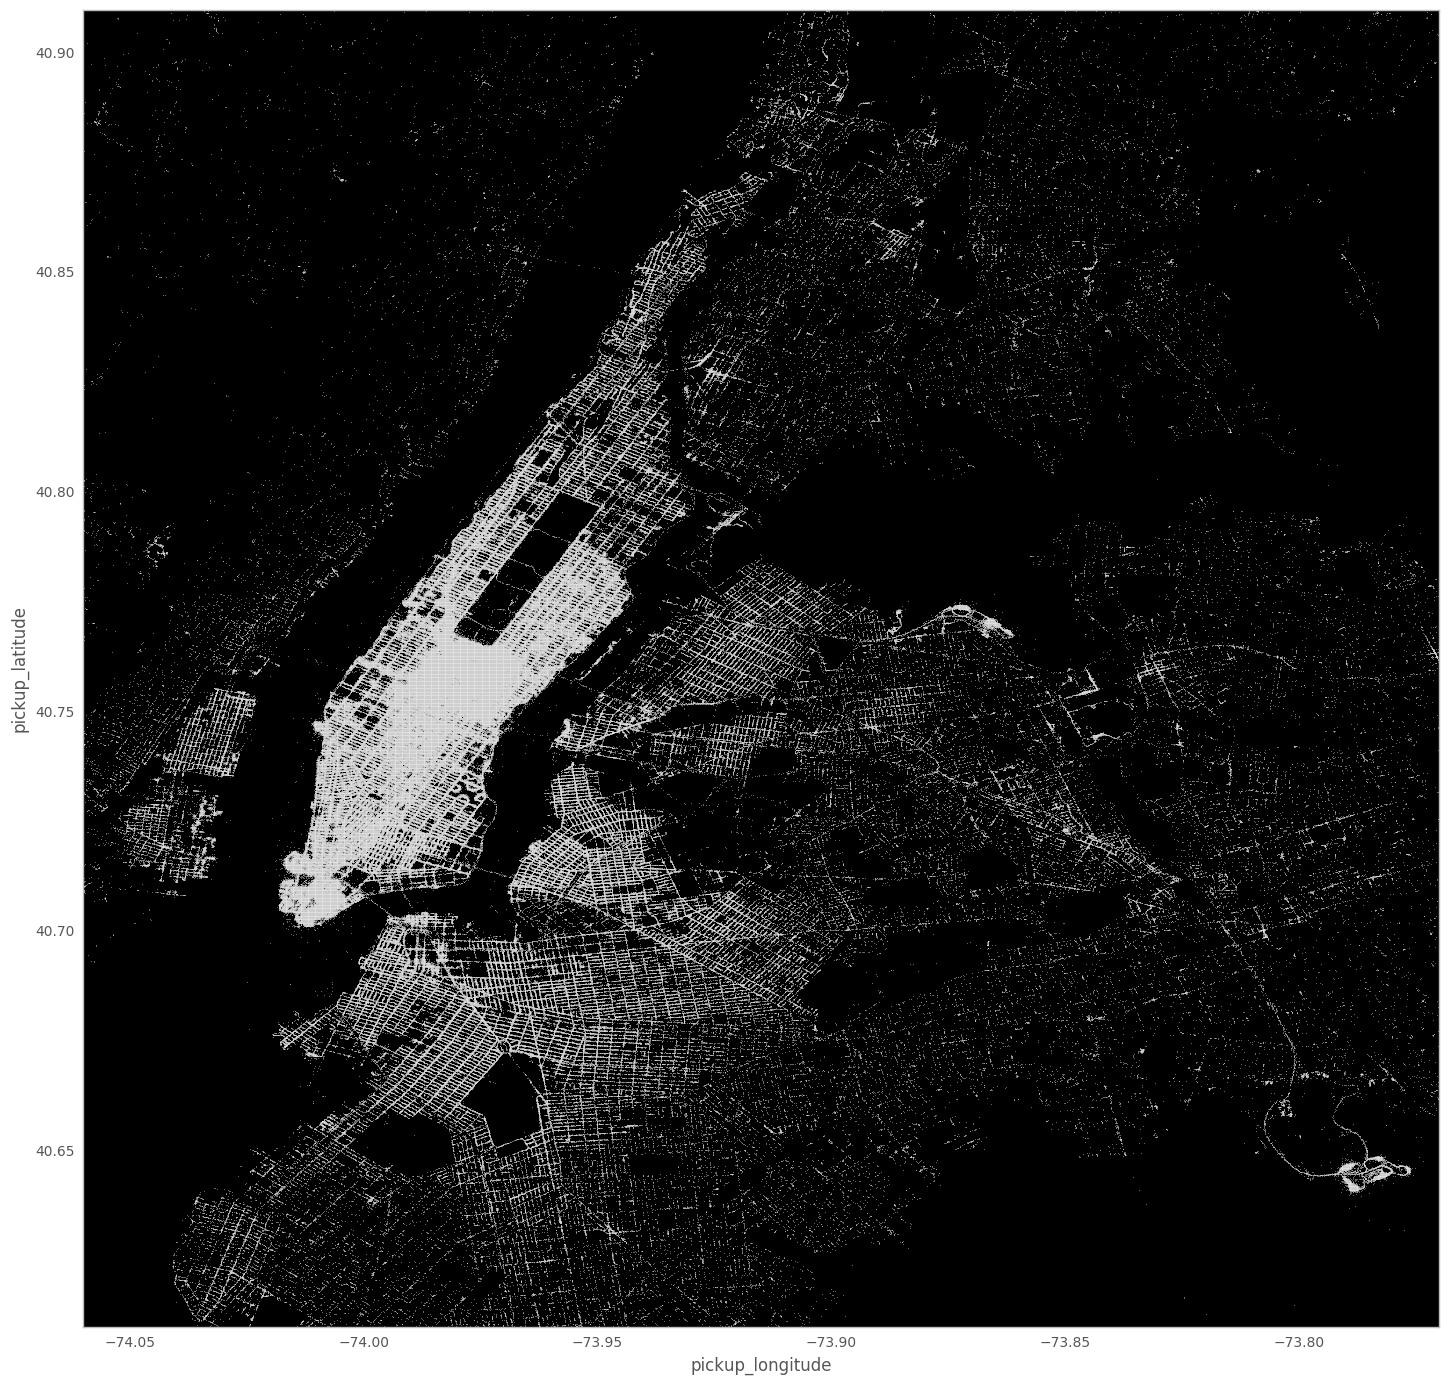
\includegraphics[width=8cm, height=8cm]{Complete.png}
\end{center}
\break

\textbf{Binning and Data Reduction}\\

The uber-dataset for all the 6 months contains around 4.5 millions records. Binning helps in reducing the number of the input required for model creation. Also it helped us in decided the label required for regression. 
Binning was done based on following creitera. \\
\begin{itemize}
\item Time based binning : All the pickup rides are divided into 24 hours slot as per pickup time.
\item Location based binning : Entire NYC areas was divided into 'n' clusters. We used spatial DBSCAN for finding this each area center point.
\end{itemize}

\textbf{Zipcode binning}\\

Initially, we wanted to do binning for lat-long based on zipcode. So we converted each lat-long point to 3-decimal precision, to reduce the file size. If we round to 3 points after decimal, we are considering all points in 100m area as a single point. There are two main issues with this approach. First being that we are losing precision by rounding off and second we can?t guarantee that zipcode regions are uniformly distributed areas. \\

So to solve this, we worked on doing manual binning by actually dividing NYC into square grids. How this approach works is we divide the city into smaller square blocks of grids and all pickup locations in that particular grid can be denoted or represented by a center of the grid. \\

We need to do one main change to this before we proceed with this step. We need to convert lat-long point into 3-dimensional point which represents the lat-long in real world. Technically we are looking at a cube space which includes all of NYC. This approach became too much technical and complex due to conversions and re-conversions. \\

We came up with a new approach for binning, that is to do a geospatial DBSCAN. So what we did was run a DBSCAN on the lat-long points to determine clusters. We didn?t use euclidean distance for distance measure, instead we went with haversine formula for calculating distance between pair of lat-long points. We did a small change to DBSCAN to find all the centers of the clusters and then represent all points belonging to the cluster by that center point. \\

\textbf{Binning by Time}\\

To work on the data and analyze the trends based on time we need to understand on how to bin the data based on 4 dimensions i.e lat, long, date and time(1 - 24). We won?t be considering minutes and seconds, as the granularity of that level wouldn?t give any useful trends. So now if we are to consider all distinct lat-long points rounded to 3 decimal, we have 6,48,517 points. We have 30 days per month and 24 hours per day. So if we were to generate all possibilities we end up with 6,48,517 * 30 * 24 records which is pretty high number to compute upon. To tackle this situation we have to come up with a binning on count. We can?t do binning on day or time as they are granularized to the maximum. We are left with lat-long points. Rounding off lat-long points to less than 3 decimal points will lead to huge loss of precision. So similar to above, we do DBSCAN to calculate grids and represent all points in cluster by center of the cluster. So now the computation complexity depends on how many grids or clusters we pre-decided. In this way, we reduce the computation complexity of the problem while still maintaining the distribution of the data. \\

\textbf{Plotting GeoJSON}\\ 

To understand the distribution of pickups across the New York city and to choose the best clustering algorithm for binning and reducing number of rows we chose to plot the pickups on GeoJSON. \break
GeoJSON is a format for encoding a variety of geographic data structures. \break
Advantages of GeoJSON in our project : Helped us understand the granularity at which we can bin our pickup latitude and longitude. Every GeoJSON point at specific zoom levels displays the number of pickups at that point. \break
Scripts to create our GeoJSON given a list of pickup lat long : \\
\begin{itemize}
\item GeoJSONCreator.sh : Script to convert our lat long to GeoJSON.
\item jsontogeo.py : Python program to convert JSON to GeoJSON.
\end{itemize}

GeoJSON of our entire dataset : \href{https://github.com/msabhi/mining-uber-dataset/blob/master/Milestone-2/Data_Plot.geojson}{GeoJSON} \\ 
After experimenting at different levels of our GeoJSON, we were able to determine the parameters for our GeoSpacial DBSCAN algorithm - \href{https://github.com/msabhi/mining-uber-dataset/blob/master/Milestone-2/GeoSpatial-DBScan-UBER.ipynb}{Code} \\
April binned points GeoJSON : \href{https://github.com/msabhi/mining-uber-dataset/blob/master/Milestone-2/binning_centers_april.geojson}{GeoJSON} \\ 
	 
\textbf{Gaussian Process Regression}\\

Training data are D = { $x^{i}$  ,$y^{i}$ $\mid$ i = 1, . . . , n}. 

\begin{itemize}
	\item Our training data for Uber is an input vector x of 4 dimensions that is latitude, longitude, date and time. 
	\item Each target is a real valued scalar y = f (x) + noise. Here f(x) is number of pickups for us
	\item Collect inputs in (d x n) matrix in X, and targets in vector, \\ 

	\centerline {Y: D = \{X, Y\} }

	\item We wish to infer f * (number of pickups) for unseen input x * , using P(f * $\mid$  x* , D). So, for any unseen input given coordinates (latitude and longitude), date, time and the training data.


\item This is an (n x d) dimensional feature map $\Phi$  

\begin{center}
$
\Phi = 
\begin{bmatrix}
. & . & \overrightarrow{\phi}(X_{1})^{T} &.  & .  &\\ 
. & . & \overrightarrow{\phi}(X_{2})^{T} &.  & .  &\\ 
. & . & .&. & . & \\ 
. & . & . &.  & .  & \\ 
. & . & \overrightarrow{\phi}(X_{n})^{T} &.  & .  & 
\end{bmatrix}
$ 
\end{center}

\item A Gaussian process is a collection of random variables, any finite number of which have a joint Gaussian distribution. $\Phi$ is (n x d) dimensions and $\phi$ is (1 x d) i.e one row of feature map. K defines joint distribution over function values. Therefore GP specifies a distribution over funtions   

\begin{center}
$K_{nm} = \lambda ^{-1} \left ( \Phi \Phi ^{T} \right )$ \break

$K_{nm}  = \frac{1}{\lambda } \overrightarrow{\phi }\left ( \overrightarrow{X_{n}} \right )^{T}\overrightarrow{\phi }\left ( \overrightarrow{X_{m}} \right ) $ \break

$K_{nm} = \frac{1}{\lambda } l\left [ \overrightarrow{X_{n}},\overrightarrow{X_{m}} \right ]$ \break

\end{center}

\item Here K is our Kernel Matrix $\Phi$  

\begin{center}

$ K := \phi \phi ^{T}$ \break

\end{center}

\item As per Linear Rigression feature map is:: \\

\begin{center}
\(\theta\)   = $(XX^{T})^{-1}X^{T}Y$ 

\end{center}



\item Maximum a Posteriori (Expected Values of Weights) D X D inversion \\

\begin{center}

$E\left [w/y  \right ] =  A^{-1}\phi ^{T}Y$\ 
\tab
$A = (\phi^{T} \phi + \lambda I )$ \break
\end{center}

\item Maximum a Posteriori (Expected Values of Weights) N X N inversion \\
\begin{center}
$K =  \lambda ^{-1} \left ( \Phi \Phi ^{T} \right )$ 
\tab
$A^{-1}\phi ^{T} = \phi ^{T}\left ( K + \lambda I^{-1} \right )$ \break
\end{center}
\item Predictive Posterior using Kernels
\begin{center}


$E\left [ f\left ( x\star  \right ) \mid y \right ] = \phi \left ( x\star  \right )^{T}E\left [ w/y \right ]$ \\

${\mathbb{E}}[\frac{f(x_{\star })}{y}] =  \phi (x_{\star })^{T}{\mathbb{E}}[\frac{w}{y}]$ 

${\mathbb{E}}[\frac{f(x_{\star })}{y}] =  \phi (x_{\star })^{T}\Phi^{T}(K + \lambda I)^{-1}y$

${\mathbb{E}}[\frac{f(x_{\star })}{y}]  = \sum_{n,m}k(x_{*},x_{n})(K + \lambda I)^{-1}_{nm}y_{m}$
\end{center}

\end{itemize}

\break

\textbf{Random Forest Regressor} \\

\textbf{Introduction} \\

In random forests each tree in the ensemble is built from a sample drawn with replacement from the training set. In addition, when splitting a node during the construction of the tree, the split that is chosen is no longer the best split among all features. Instead, the split that is picked is the best split among a random subset of the features. As a result of this randomness, the bias of the forest usually slightly increases but, due to averaging, its variance also decreases, usually more than compensating for the increase in bias, hence yielding an overall better model.

\textbf{Pre-processing Step}

To use our data with Random Forest regressor, we did few steps of pre-processing. 

\begin{itemize}
	\item Grid Binning
	\item Epoch Time Conversion
	\item Binning by Time+Grid
\end{itemize}

Grid binning is the way of binning in which we divide the entire area of NYC into equally spaced uniform square grids. We do binning by considering all latitude and longitude points lying in a grid and then represent them by grid itself. We represent the grid by row and column it belongs to. This way we can reduce the size of data points but still maintain the original distribution of the data.
Now we have to find a centre to represent the grids itself. Original way to do this to find the mean of all the points in the grid and use that point for representation. We did in a simpler way by just using grid numbers to represent the grid itself. Why this works as original is because grid numbers are also equally spaced and uniformly distributed as the original centers. 
Doing so, gave us a clear picture of how NYC looks in grids. Here is the picture on 1000x1000 grids.


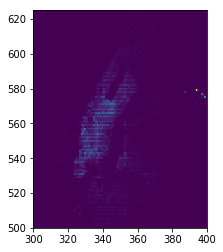
\includegraphics[width=8cm, height=8cm]{binning.png}

We can make out the outline of Manhattan from this HeatMap. We can go more granular by increasing the grids, but that would outdo the reason why we did binning on first place.
We did binning on 100x100 grids, but that didn?t give us a clear picture nor accuracy we expected.

\textbf{Epoch Time Conversion }

The Unix epoch (or Unix time or POSIX time or Unix timestamp) is the number of seconds that have elapsed since January 1, 1970 (midnight UTC/GMT), not counting leap seconds (in ISO 8601: 1970-01-01T00:00:00Z) 
The reason why we did this is to convert the standard date-time format to a number format, as it acts as one of the input feRandom Forest Regressor.

\textbf{Binning on Time}

We bin on time and grid together and find counts for each unique combination. Time here is just counted on hours, not minutes and seconds as we won?t be getting meaningful trends in that granularity. We use the count as Y label for random forest regressor(estimator).

\textbf{Results}

Prediction accuracy was 89 with Random Forest Estimator. We used 5 months starting from april to august as training data and September data as testing data. We used a mean error of 1(2 was the standard deviation of the original data) ride for finding the accuracy.  \\

\textbf{Prediction Accuracy =  89} \\
\textbf{Root Mean Square Error =  1.7914}

\textbf{Trends}

We wanted to find trends on this. Let?s see how Friday evening differs from Monday morning.

\break

\textbf{REFRENCES:} \\
\begin{itemize}
\item \href{https://www.linkedin.com/pulse/amazing-ways-uber-using-big-data-analytics-bernard-marr}{https://www.linkedin.com/pulse/amazing-ways-uber-using-big-data-analytics-bernard-marr}
\item \href{http://geojson.org/}{http://geojson.org/}
\end{itemize}
\end{document}